%!TEX root = umthsmpl.tex
\chapter{Location privacy threats from a streaming service}
This chapter explores the threats to location privacy when a user downloads data while in motion, and presents an evaluation on the loss of utility if a user attempts to reduce these threats\footnote{This chapter is based on work published at the Privacy Enhancing Technologies Symposium\cite{soroush2013turning}}. I propose to analyze in more detail some algorithms more suited to this problem, and the trade-offs between traffic-shaping to preserve privacy and utility.

\section{Preliminary work: Identifying the path traveled using throughput}

Despite features on smartphones to ensure location privacy, a user's whereabouts can be remotely deduced. A remote party communicating with a phone has a window into the complex interactions between phone and cell tower. These features can be used to reveal the phone's location, or at least significantly narrow the list of possible paths taken by a phone and its owner. This information is leaked regardless of application-level privacy settings. Cell phone users have such experiences intuitively in many common situations. For example, a caller may be able to tell when a friend has entered an elevator based solely on call quality; or a user may notice a loss in data throughput during a subway ride.

We collected hundreds of traces of music that we streamed to 
phones along four geographically separate routes in two 
directions each.  We find that within small geographical areas,  
mean throughput is largely consistent and distinct. We examine 
the accuracy of three
remote localization classifiers that leverage this consistency. 
Even a naive approach, trained on the mean throughput of each path, 
has some success. 
We compared this classifier against a
$k$-nearest neighbors ($k$-NN) classifier, which trains on the ordered
sequence of throughput values of each rout, a hidden Markov model
(HMM) classifier, which exploits the consistency in throughput values
at each location, and a Naive Bayes (NB-KDE) classifier that uses
kernel density estimation of throughput at each second along a path.
Our best performing approach, the NB-KDE classifier, can correctly
determine with greater than the path taken by the phone from one of
four longer paths to neighboring suburbs with greater than 90\%
accuracy, and the path and direction (8 choices) with 76\%
accuracy. In a separate experiment involving data collected only from
within a 4km$^2$ area, in and around our campus, the NB-KDE approach
could identify the direction and part of campus the user was traveling
with 76\% accuracy.

\paragraph*{Data}
Our measurements\footnote{Traces from our experiments are available for download from \url{http://traces.cs.umass.edu}.}
are based on four Android cell phones instrumented to record traces of GPS location and 
signal strength. %, and tower association.  
A server in our building streamed music 
continuously to the phones during measurement trials. We logged TCP traces at the server during trials. We later combined sets of corresponding phone and server traces, synchronizing by the timestamps within the traces. 

\begin{itemize}
	\item {\bf Mobile 3G Measurement Set --- Paths to Towns}: We used four phones connected to the AT\&T UMTS (3G)
	network to record traces. We collected data during a
	one-month period under varying traffic and weather conditions. Each
	measurement was taken as a phone traveled along one of four routes
	going either toward or away from our central location (point X in
	Figure~\ref{fig:map}). In total, we recorded 286 traces in
	this set.
	\item {\bf Mobile 3G Measurement Set --- Paths within Campus}: We
	recorded 141 traces from the same phones, along one of two
	directions around a bus loop on campus. Traces were collected over a
	period of eight months.
	\item {\bf Stationary 3G Measurement Set}: We recorded 29 traces from
	stationary phones, connected to the UMTS (3G) network, located in
	different locations near our central location.
\end{itemize}

\begin{figure}%[p]
	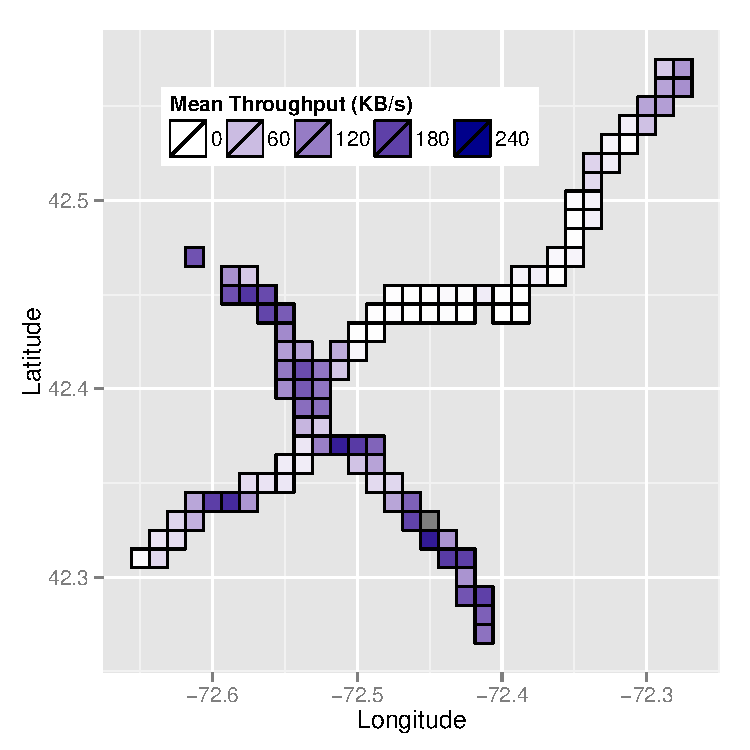
\includegraphics[width=0.5\textwidth]{graphics/amherst_tput_map.pdf}
	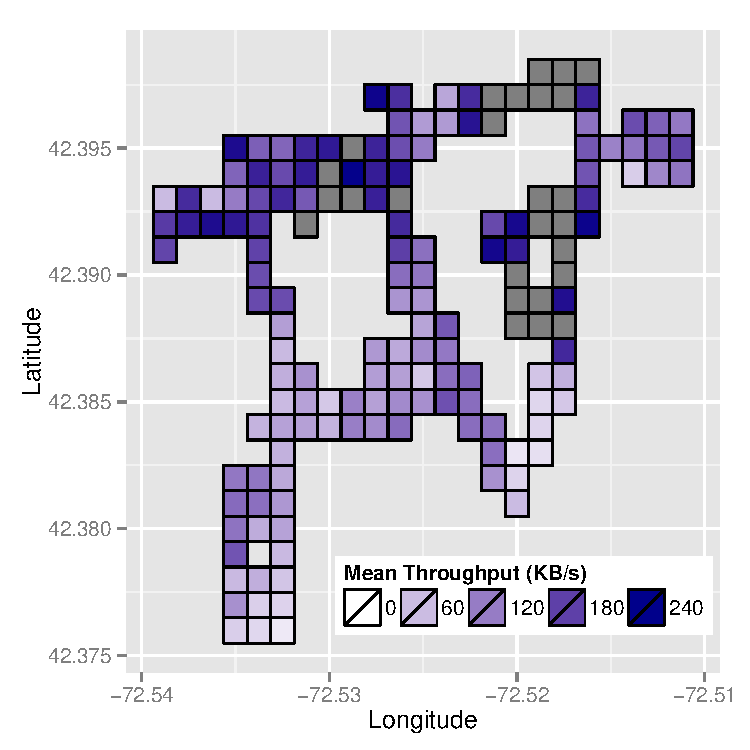
\includegraphics[width=0.5\textwidth]{graphics/umass_tput_map.pdf}
	\caption{The mean throughput of locations around Amherst (left) and
		within UMass (right). 95\% of areas have means that are statistically different from at least 90\% of other areas. This data suggests that latent information linking throughput and geography is available for training a classifier. }
	\label{fig:map}
\end{figure}

\paragraph*{Algorithms}
I present a hidden Markov model (HMM), $k$-nearest neighbors ($k$-NN),
and naive bayes (NB-KDE) classifier with respect to a motion-throughput
model. Each classifier is derived from this model, with different assumptions. The HMM classifier is most general, and attempts to maximize the estimated hidden states and transitions. The $k$-NN and NB-KDE classifiers are more rigid, and make the assumption that users move through a certain path with consistent velocity. The $k$-NN classifier finds
$k$ of the closest traces by comparing the throughput at each time
point of the trace. The NB-KDE classifier determines the distribution
of throughputs at each time point for each path, and finds the most
likely trace.

In our evaluation, we tested the identification of a path rather than
a sequence of locations. Therefore, we have split the location sequences
into separate path classes. 

For the HMM, The states are fixed as approximate square areas on the map. Emission
probabilities at each state are determined by counting the number
of occurrences of each throughput level in the training data in each
area and normalizing. A throughput level $e=0\dots15$ for 16 throughput
levels. The probability of a certain throughput level occurring at
a certain location is from a categorical distribution:

\begin{equation}
p(e|l)=\sum_{j\in N_{l}}[\mathcal{M}(o_{j}^{l})=e]/N_{l},
\end{equation} where $\mathcal{M}$ maps a throughput value $b$ to an emission level $e$ depending on which fixed range it is between.

The Markov assumption~\cite{markov1957theory} allows us to consider the probabilities of each transition independently: 
\begin{align}
p(\mathbf{l}|\mathbf{b})&=p(l_{0}|b_{0})p(l_{1}|b_{1},l_{0}),p(l_{2}|b_{2},l_{1},l_{0})\dots\\
p(l_{t}|b_{t},l_{t-1},l_{t-2},\dots,l_{0})&=p(l_{t}|b_{t},l_{t-1})\\
p(\mathbf{l}|\mathbf{b})&=\prod_{t}p(l_{t}|b_{t},l_{t-1})\\
p(\mathbf{l}|\mathbf{b})&=\prod_{t=1}^{|\mathbf{b}|}p(l_{t}|l_{t-1})p(b_{t}|l_{t})
\end{align}

For the sequence-based $k$-NN and NB-KDE, we assumed that subjects travelled
along the path at consistent speeds. Recall that for the $k$-NN and
NB-KDE, $\mathbf{c}=l_{0},l_{1},\dots$ represent a virtual location
for each second along a path, rather than directly mapping to a geographic
location.

For the $k$-NN, we compute a distance between the test trace $\mathbf{b}$
and training traces $\mathbf{b}^{tr}\in B^{tr}$, as
\begin{align}
\mathrm{distance}(\mathbf{b},\mathbf{b}^{tr})=\sum_{t=0}^{|\mathbf{b|}}|\mathbf{b}_{t}-\mathbf{b}_{t}^{tr}|.
\end{align}

Subsequently, we rank the sequences $\mathbf{b}^{tr}$ by the computed
distance from lowest to highest. We classify the instance as the label (i.e., the route) present in the largest 
fraction of the $k$-nearest neighbors. If there is a case of a tie,
we increment $k$ for that case until the tie is broken.

For the NB-KDE classifier, we determine
\begin{align}
\arg\max_{\mathbf{c}}p(\mathbf{c}|\mathbf{b}).
\end{align}

\noindent
Each location is associated with a kernel density estimator, with
Gaussian kernel $K$:
\begin{align}
f(b|l)=\frac{1}{N_{l}}\sum_{i=0}^{N_{l}}K(b-b_{i}^{l})
\end{align}

\noindent
We use the KDE to estimate the probability of a certain bandwidth
at a location, so that
\begin{align}
p(b_{t}|l_{t})=f(b_{t}|l_{t}).
\end{align}
Therefore,
\begin{align}
\arg\max_{\mathbf{c}}p(\mathbf{c}|\mathbf{b})=\arg\max_{\mathbf{c}}\prod_{t=0}^{|\mathbf{c|}}f(b_{t}|l_{t}^{\mathbf{c}}).
\end{align}

\paragraph*{Evaluation}
We evaluated the classifiers above with different scenarios using 3-fold cross-validation for hyperparameters, and leave-one-out cross-validation during training. In general, the NB-KDE classifier performed the best. The HMM classifier performed poorly, because the errors in predicting speed variations propagate as the trace gets longer. Results for every experiments are shown in Table \ref{table:mobile-accuracy}.

\begin{table}
	\centering
	\begin{tabular}{lcccccc}
			\hline {\textbf{Experiment}}&
			{\textbf{Classes}}&
			{\textbf{NB-KDE}}&
			{\textbf{k-NN}}&
			{\textbf{HMM}}&
			{\textbf{Tput}}&
			{\textbf{Freq}}\\
			\hline \hline
			4 paths$\times$ 1  (Outward)   & 4 & {\bf 90.3} & 51.4 & 18.8 &7.3 &36.6\\
			4 paths$\times$ 1  (Inward)    & 4 & {\bf 83.3} & 43.9 & 42.4 & 3.7 &28.6\\\hline
			4 paths (Western MA)$\times$ 2 & 8 & {\bf 75.7} & 25.4 & 26.1 &1.7&20.4\\\hline
			2 paths (UMass)$\times$ 2      & 4 & 75.8 & {\bf 77.6} & 53.3 &12.4& 44.7\\
			\hline
	\end{tabular}
	\caption{Classification accuracy depending on which roads are included in the experiment. Bolded entries have the highest accuracy.}
	\label{table:mobile-accuracy}
\end{table}

The NB-KDE classifier performed relatively well with short traces, as shown in Figure \ref{fig:tputlen}. Both the $k$-NN and NB-KDE classifiers increased in accuracy as length increased. This shows that while decreasing the length of the connection to the server does increase user privacy, it may not be enough; other traffic shaping options should be explored. 

\begin{figure}
	\centering
	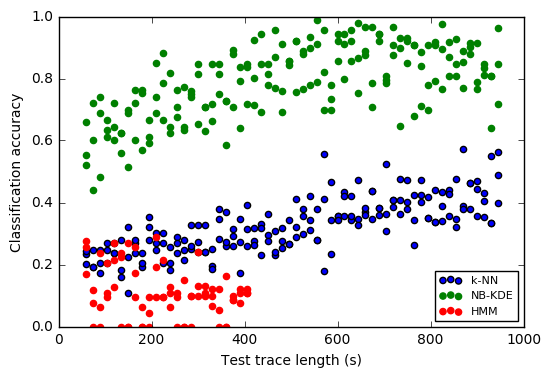
\includegraphics[width=0.7\textwidth]{graphics/tputlength}
	\caption{Accuracy of experiments (randomized test set) with varying trace lengths.}
	\label{fig:tputlen}
\end{figure}

% \section{Proposed work: Additional classifiers, and utility analyses}
\section{Proposed work}
I do not propose additional work for this chapter, though in my final dissertation, I will include a version of the work to be submitted to a journal that is more detailed than both this summary and the version presented at the \emph{Privacy Enhancing Technologies Symposium}.
%I propose to extend this work to by using more sophisticated classifiers, namely a hidden semi-Markov model \cite{johnson2013bayesian}. As well, I would use the data collected for Chapter 1 to determine the usefulness of features such as time of day (see Figure \ref{fig:tod}). Finally, I will evaluate traffic shaping algorithms by degrading the current data, and analyze utility vs privacy tradeoff for this problem. Key questions:
%\begin{enumerate}
%	\item How well would an HSMM do for this problem?
%	\item How useful are additional features such as time-of-day?
%	\item How effective are traffic shaping algorithms?
%\end{enumerate}
%
%\begin{figure}
%	\centering
%	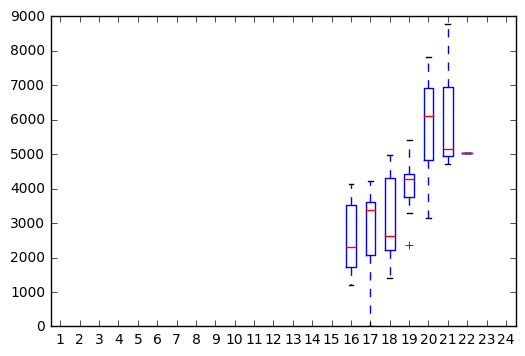
\includegraphics[width=0.4\textwidth]{graphics/noho}
%	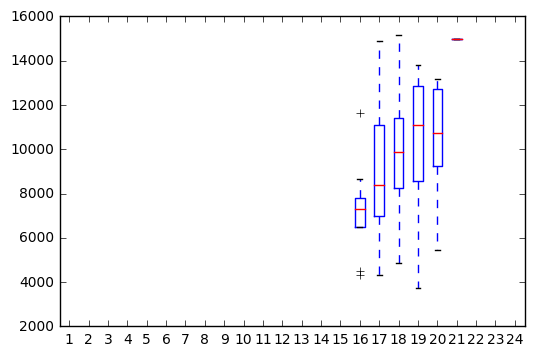
\includegraphics[width=0.4\textwidth]{graphics/sund}
%	\caption{Average throughput of trace (B/s) vs hour of day around Northampton (left) and Sunderland (right). Plots indicate a trend towards higher throughput at night.}
%	\label{fig:tod}
%\end{figure}